\documentclass[compress]{beamer}

\usepackage[utf8]{inputenc}
\usepackage{graphicx}
\usepackage{color}
\usepackage{colortbl}
\usepackage{listings}
\usepackage{caption}
\usepackage{pgfpages}
\usepackage{tabularx}
\usepackage{amsthm}
\usepackage{url}

%\usetheme[basergb={1,0.2,0.2}]{Dcon}
%\usetheme[baseRGB={23,102,34}]{Dcon}
\usetheme{Dcon} % default color

%%%%%%%%%%%%%%%%%%%%%%%%%%%%% Definitions %%%%%%%%%%%%%%%%%%%%%%%%%%%%%%%%%%%%%

\newcommand{\logotum}{
\includegraphics[scale=0.9]{TUMINF.pdf}}
\newcommand{\logoinf}{
\includegraphics[scale=0.5]{IN_schwarz_CMYK.pdf}}

\newcommand{\hl}[1]{\fcolorbox{red}{white}{#1}}
\newcommand{\todo}[1]{\hl{TODO: #1...}}
\newcommand{\review}[0]{\todo{REVIEW}}
\newcommand{\comm}[1]{\textsuperscript{\bf \color{red}{\tiny [#1]}}}
\newcommand{\q}[0]{\comm{?}}
\newcommand{\s}[0]{\comm{*}}

\newcommand{\scite}[1]{\textsuperscript{\tiny\cite{#1}}}

\bibliographystyle{apalike}


\titlegraphic{\logotum}
\title[Intelligent Learning Framework]
{Intelligent Support\\ \strut for non-linear Serious Games}
\subtitle{\scriptsize{Bachelor's Thesis in Computer Science}}
\author[Felix Kaser]{Felix Kaser\\\tiny{\texttt{kaserf@in.tum.de}}}
\institute[TUM]
{Chair for Applied Software Engineering\\
Faculty of Informatics\\
Technische Universit\"at M\"unchen}
\date{July 1, 2010}
\logo{\logoinf}
\additionaltext{\tiny
{Supervisor: Prof. Bernd Brügge, PhD.\\
\hspace{7mm}Advisors: Dipl.-Inf. Univ. Dennis Pagano,\\
\hspace{17.2mm}Dipl.-Inf. Univ. Damir Ismailović}}

%%%%%%%%%%%%%%%%%%%%%%%%%%%%% Document %%%%%%%%%%%%%%%%%%%%%%%%%%%%%%%%%%%%%%%%%

\begin{document}

% title page
\begin{frame}[plain]
\titlepage
\end{frame}

\begin{frame}{Outline}
\tableofcontents
\end{frame}

\section{Introduction}
%%%%%%%%%%%%%%% Introduction %%%%%%%%%%%%%%%%%%%%%%%
\subsection{Problem Statement}

\begin{frame}{Problem Statement}
\begin{itemize}
\item Education in general lacks technology
\item Traditional instruction is not engaging enough for the ``digital natives'' \cite{VanEck2006}
\item Design for the average user is not always the best solution \cite{Bailey1982}
%\item Educational software mostly lacks adaptive approaches
%\item Non linear games give more freedom to the learner
%\item State of the art technology can enhance learning \cite{Shute2003b}
\end{itemize}
\pause
\textbf{Enabler:}
\begin{itemize}
\item Using games in education solves the lack of motivation in instruction \cite{VanEck2006}
\item Non linear games give the player a lot of freedom and are thus more engaging (highly immersive) \cite{Seah2008a}
\end{itemize}
\pause
\begin{block}{Hypothesis:}
Detecting problems during the learning process (with a non linear serious game) and adapting the game accordingly can enhance learning even more.
\end{block}
\end{frame}

\subsection{Serious Games}

\begin{frame}{Serious Games}
\pause
\begin{itemize}
\item Higher purpose than pure entertainment
\item First mentioned in Clark Abt's book \cite{Abt1987}, not in the context of computer games
\item A more up to date (``digitalized'') definition comes from Michael Zyda \cite{Zyda2005}
\end{itemize}
\pause
\begin{block}{Serious games are ...}
``a mental
contest, played \textbf{with a computer} in accordance with specific rules, that uses
entertainment to further government or corporate training, education, health,
public policy, and strategic communication objectives.'' \cite{Zyda2005}
\end{block}
\end{frame}

\subsection{Non Linear Games}

\begin{frame}{Non Linear Games}
\pause
\begin{itemize}
\item No strict storyboard to follow
\item The player has more/full freedom
\item Highly immersive (feeling of ``being there'' \cite{Psotka1995a})
\item Educational importance: immersion supports learning \cite{Zimmerman2000a, Seah2008a}
\end{itemize}
\pause
\begin{block}{Other terms:}
Open-World Games, Open-Ended Games, Sandbox Games or Exploratory Learning Environment
\end{block}
\end{frame}

\begin{frame}{Non Linear Serious Games - Examples}
\begin{block}{Physics}
%\begin{figure}
    \centering
    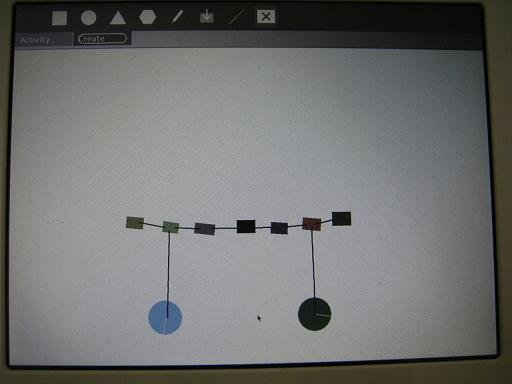
\includegraphics[width=0.3\textwidth]{images/Bridgependulum.jpg}
    \hspace{0.5em}
    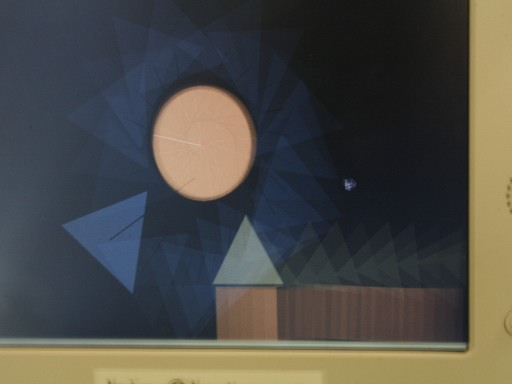
\includegraphics[width=0.3\textwidth]{images/Housegolf.jpg}
    \hspace{0.5em}
    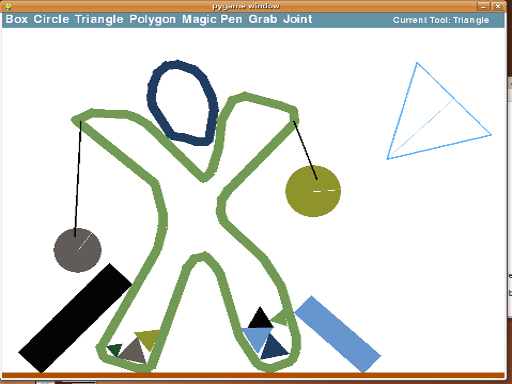
\includegraphics[width=0.3\textwidth]{images/PhysicsNew3.png}
%\end{figure}
\end{block}
\pause
\begin{block}{Food Force}
%\begin{figure}
    \centering
    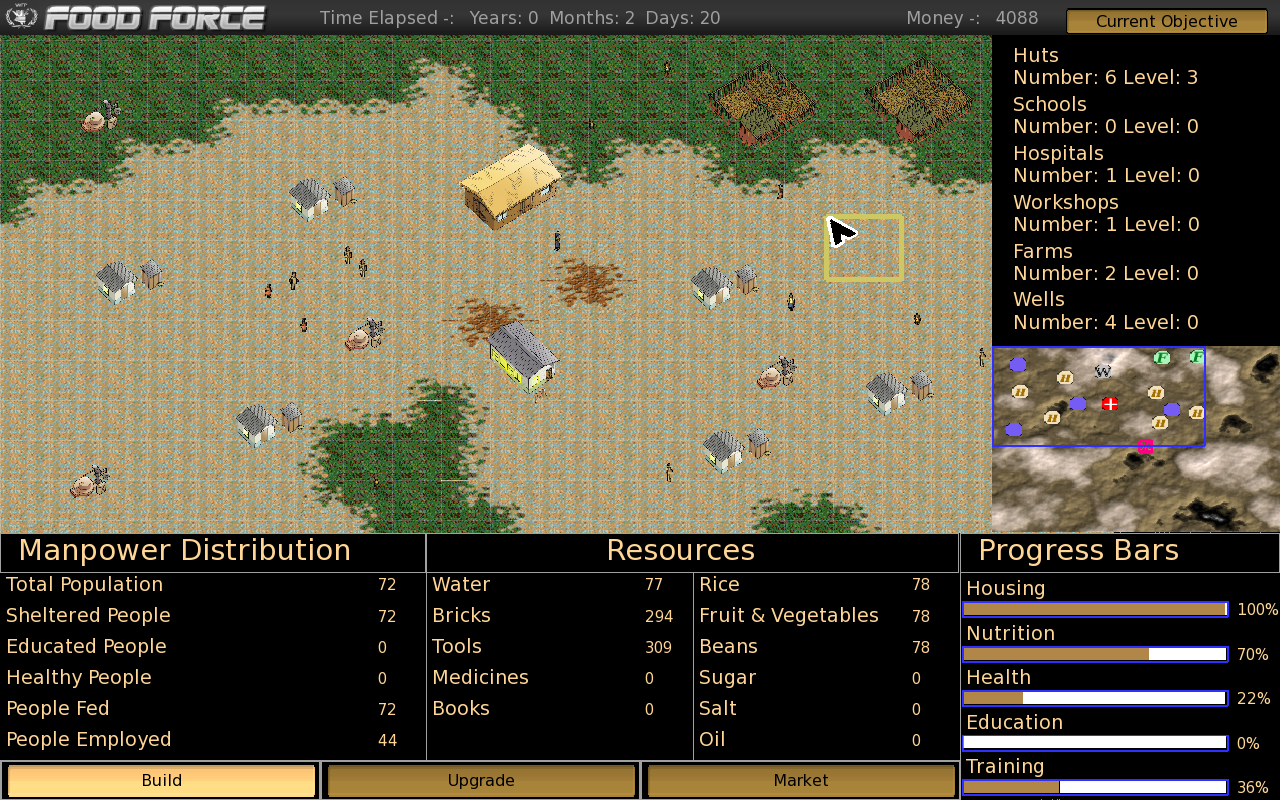
\includegraphics[width=0.3\textwidth]{images/FoodForce2_Setup_Window.png}
    \hspace{0.5em}
    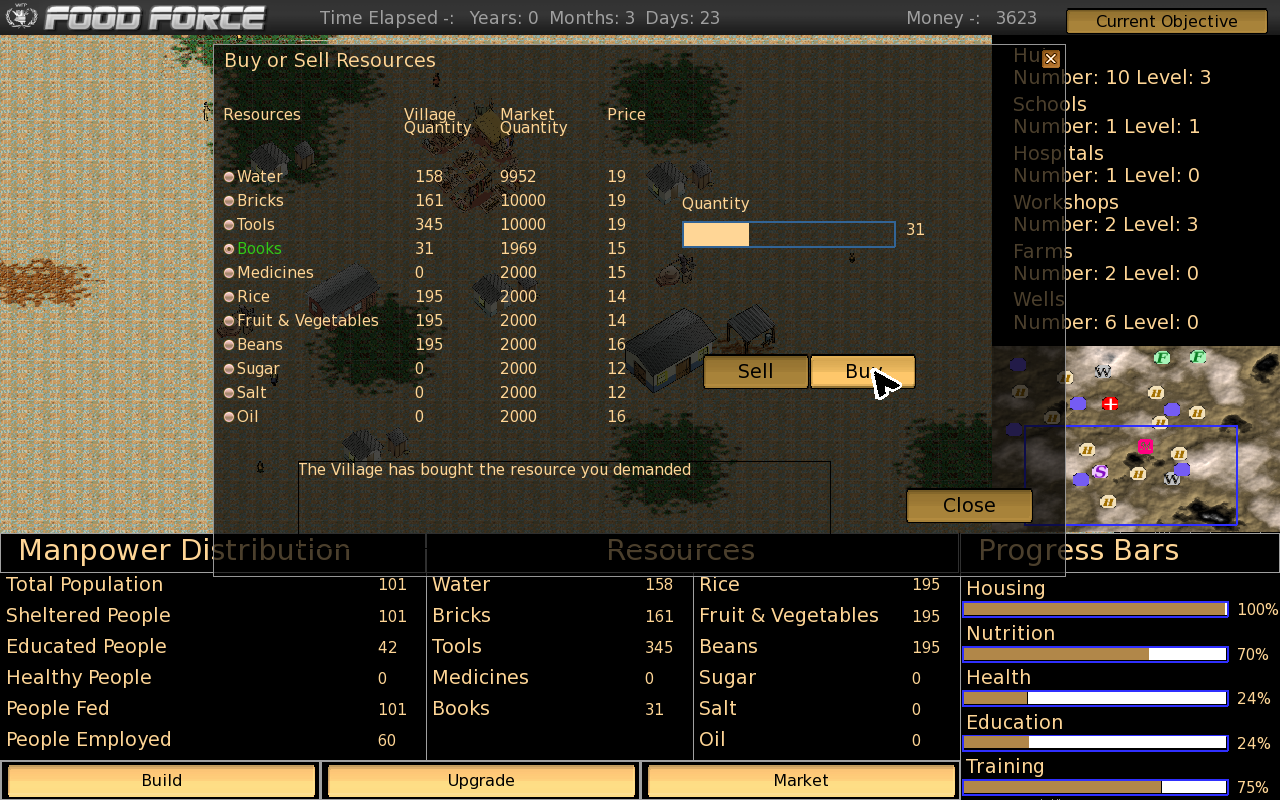
\includegraphics[width=0.3\textwidth]{images/FoodForce2_Market.png}
    \hspace{0.5em}
    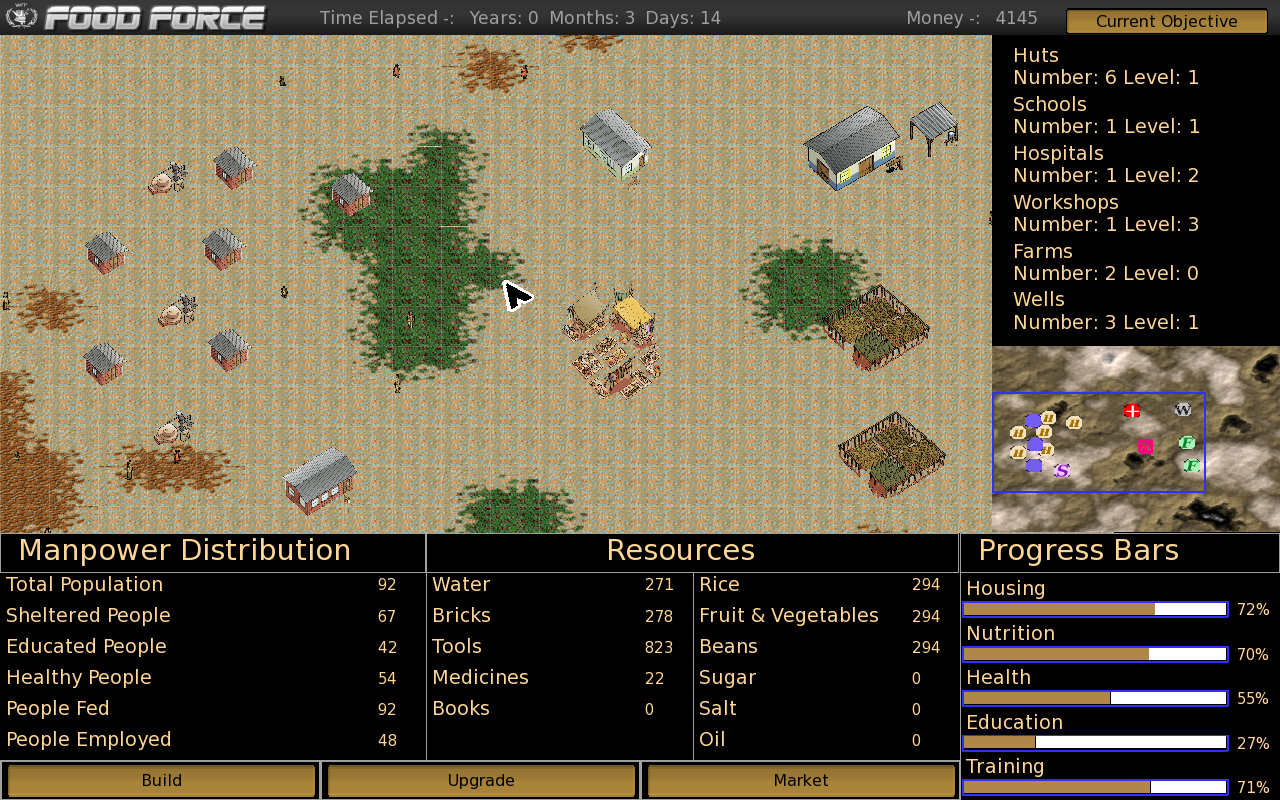
\includegraphics[width=0.3\textwidth]{images/Foodforce-mp.png}
%\end{figure}
\end{block}
\end{frame}

\subsection{Pedagogical Agents}
\begin{frame}[allowframebreaks]{Pedagogical Agents}
\begin{figure}[t]
    \centering
    \includegraphics[width=0.7\textwidth]{../latex/images/pedagogical_agent.jpeg}
    \caption[Herman the Bug, a Pedagogical Agent]
    {Herman the Bug, a Pedagogical Agent \cite{Lester1997c}}
\end{figure}
\end{frame}
%\framebreak

\begin{frame}%{Pedagogical Agents}
\begin{block}{Pedagogical agents are widely researched in terms of:}
\begin{itemize}
\pause
\item \textbf{appearence} \cite{Johnson2000, Slater2000a, Voerman1997a}
\pause
\item \textbf{interaction} \cite{Slater2000a, Baylor2003b}
\pause
\item \textbf{learning enhancements} \cite{Conati2004b, Baylor2003b, Blanchard2004b, Voerman1997a}
\pause
\item \textbf{support for artificial intelligence} \cite{Nunes2002b}
\end{itemize}
\end{block}

\pause

\begin{block}{Moreno et al.}
Pedagogical agents can ``promote constructivist learning in a
discovery-based learning environment''\cite{Moreno2000a}
\end{block}
\end{frame}

\section{Intelligent Learning Framework}
%%%%%%%%%%%%%%%% ILF section %%%%%%%%%%%%%%%%%%%
\subsection{Overview}

\begin{frame}{Intelligent Learning Framework}
\pause
Goals:
\begin{itemize}
\item Collect and analyze the learners actions during gameplay
\item Detect problems and general behavioral patterns
\pause
\item Give feedback to the learner
\item ``Support'' the learning process
\item Allow different pedagogical approaches
\end{itemize}
\end{frame}

%\begin{frame}{System Overview}
%how it connects with the game
%\end{frame}

\subsection{Analysis}

\begin{frame}{Use Cases}
\begin{figure}[t]
    \centering
    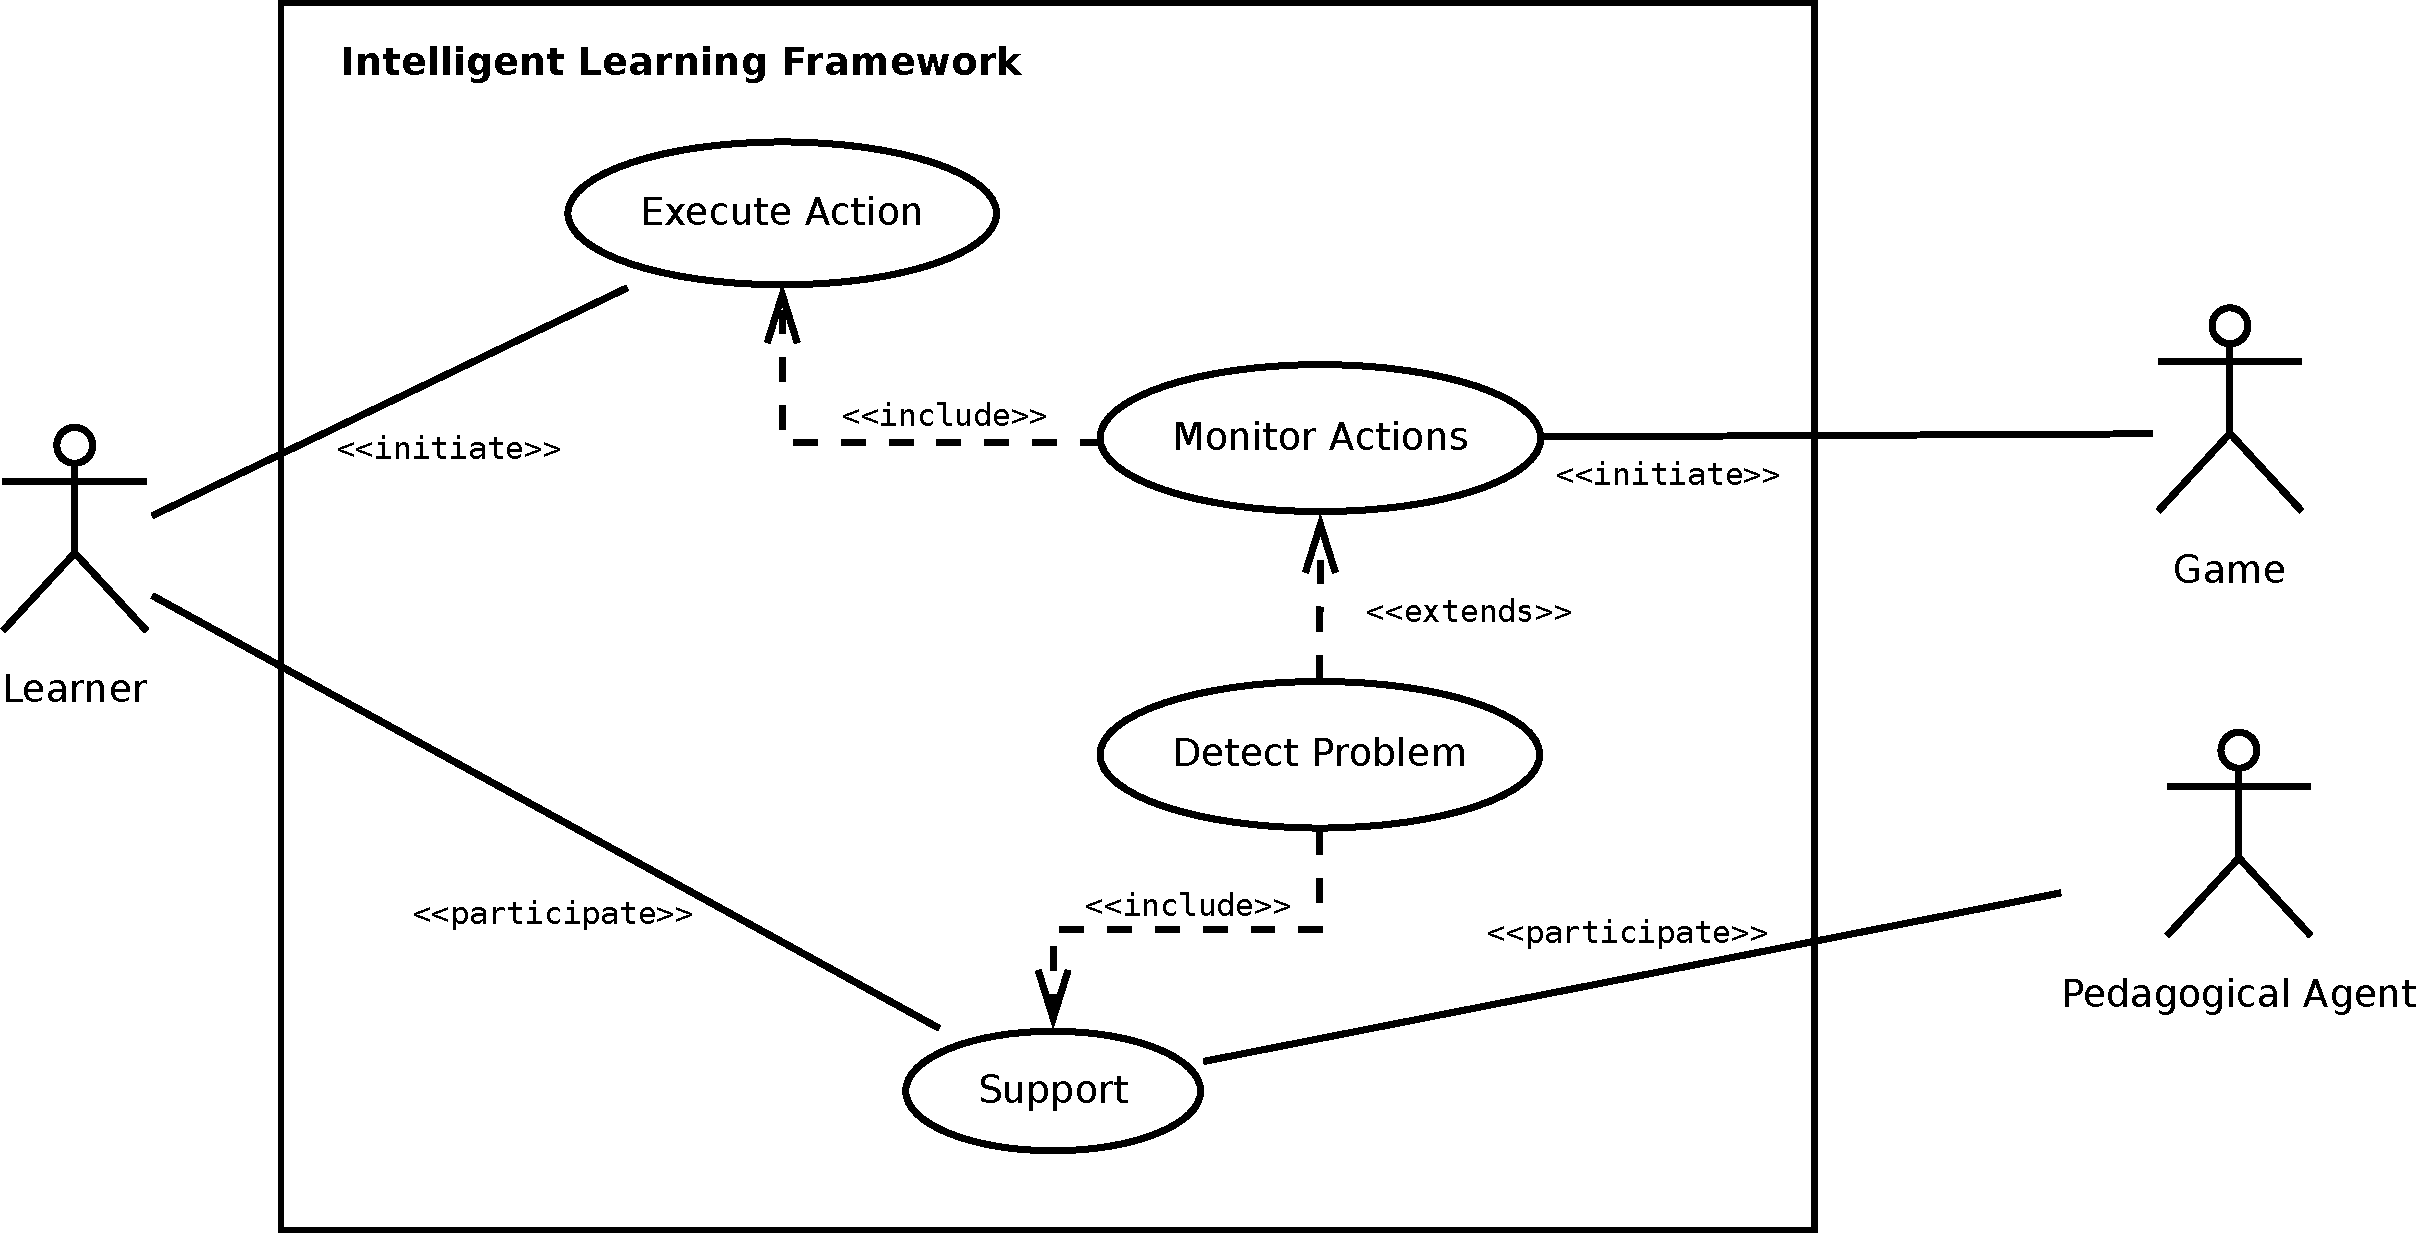
\includegraphics[width=0.9\textwidth]{diagrams/simple_use_case.pdf}
    \caption[Main use cases (UML use case diagram)]
    {Main use cases (UML use case diagram)}
\end{figure}
\end{frame}

\begin{frame}{Flow of Events}
\begin{figure}
    \centering
    \includegraphics[height=0.8\textheight]{../latex/diagrams/flow_of_events.pdf}
    \caption[Exemplary Flow of Events (UML sequence diagram)]
    {Exemplary Flow of Events (UML sequence diagram)}
\end{figure}
\end{frame}

\begin{frame}[allowframebreaks]{Action, Interaction and Event}
\begin{figure}
    \centering
    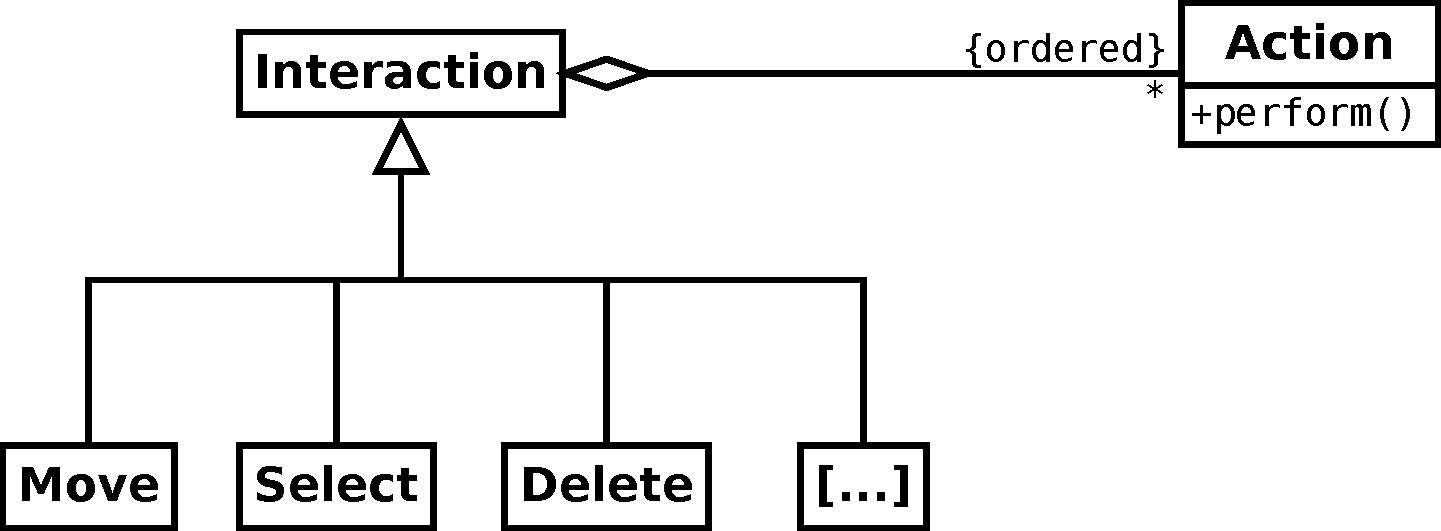
\includegraphics[width=\textwidth]{diagrams/action_interaction_simple.pdf}
    \caption{Relation between Interaction and Action (UML class diagram)}
\end{figure}

\begin{figure}
    \centering
    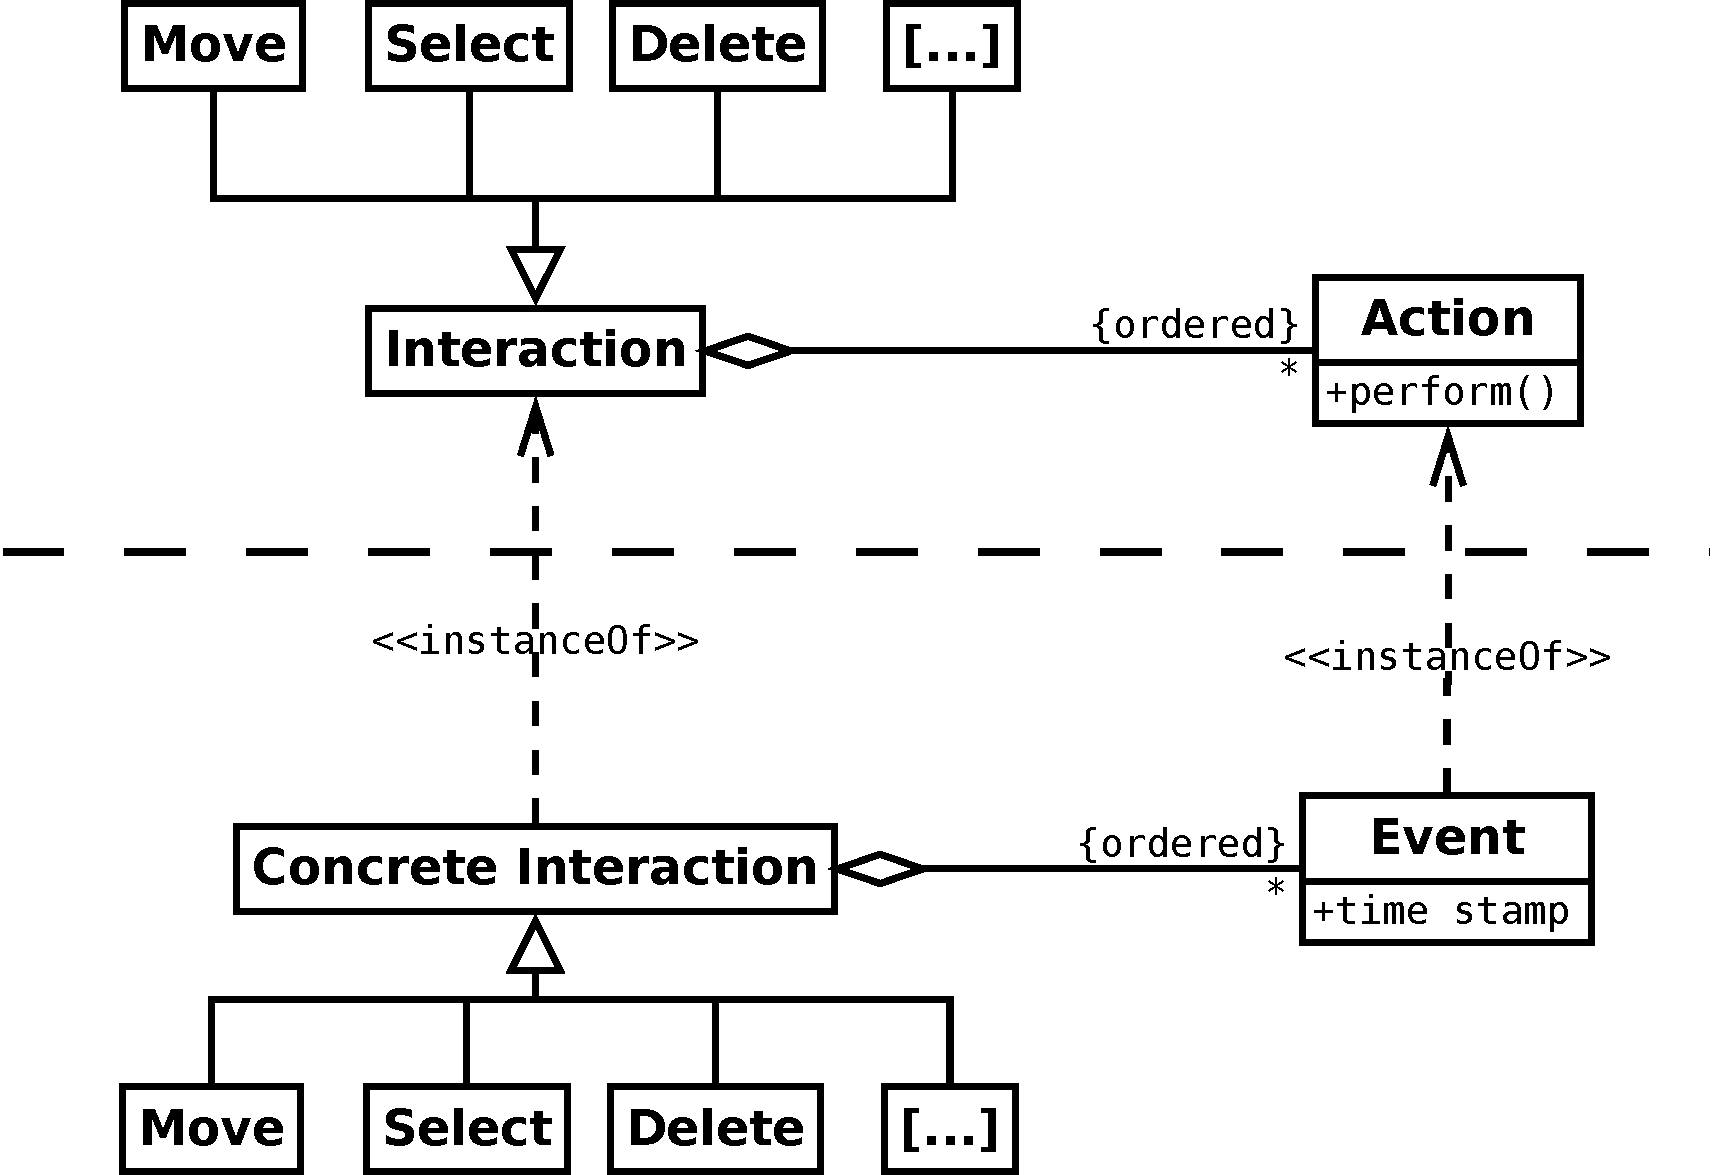
\includegraphics[height=0.6\textheight]{diagrams/action_interaction_complex.pdf}
    \caption{Different meta levels (UML class diagram)}
\end{figure}
\end{frame}

%\begin{frame}{Flow of Events}
%flow of events through the system
%\end{frame}

\begin{frame}{Problem Detection}
\begin{figure}
    \centering
    \includegraphics[width=\textwidth]{../latex/diagrams/problem_detection_process.pdf}
    \caption{The Process of Problem Detection (UML activity diagram)}
\end{figure}
\end{frame}

\subsection{System Design}

\begin{frame}[allowframebreaks]{Subsystem Decomposition}
\begin{figure}
    \centering
    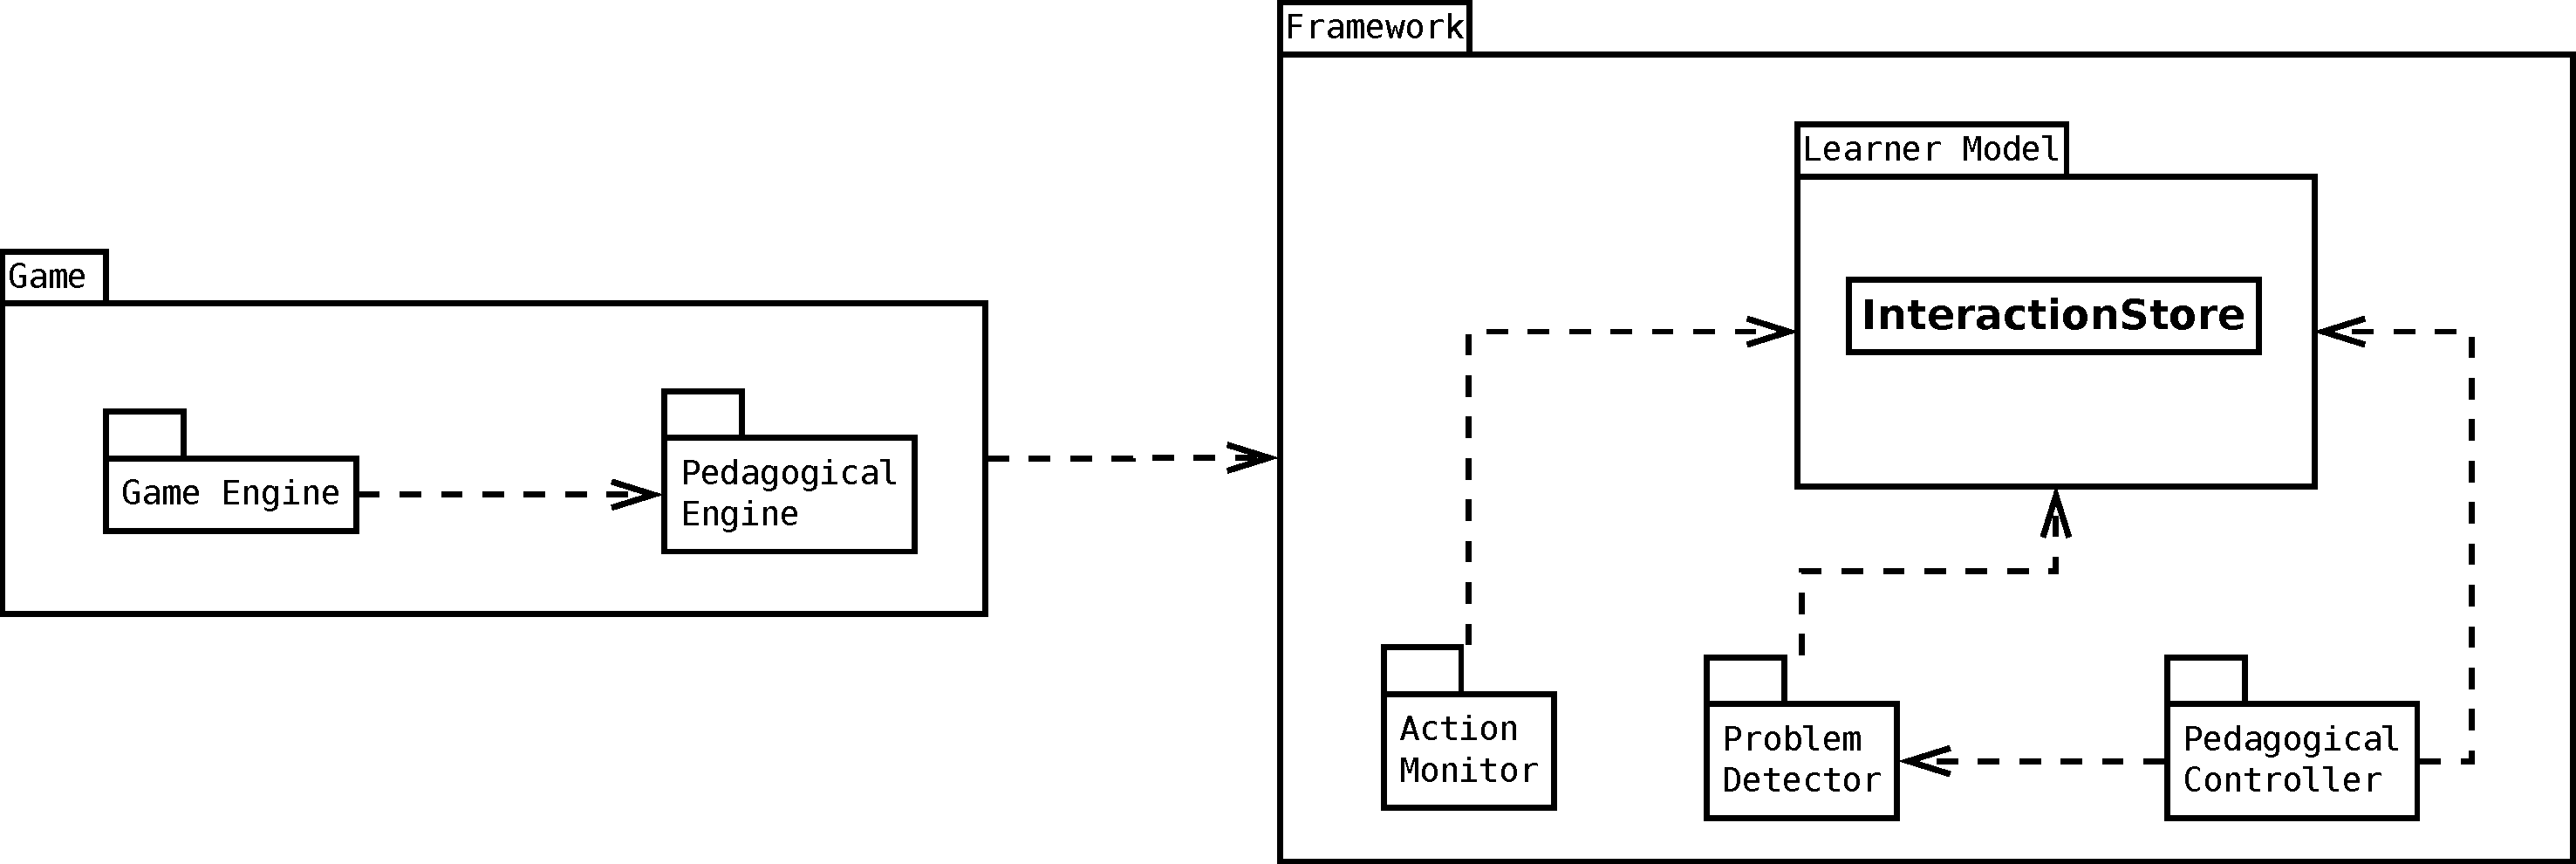
\includegraphics[width=1.05\textwidth]{diagrams/subsystem_decomposition_new.pdf}
    \caption{Subsystem Decomposition Overview (UML package diagram)}
\end{figure}

\begin{figure}
    \centering
    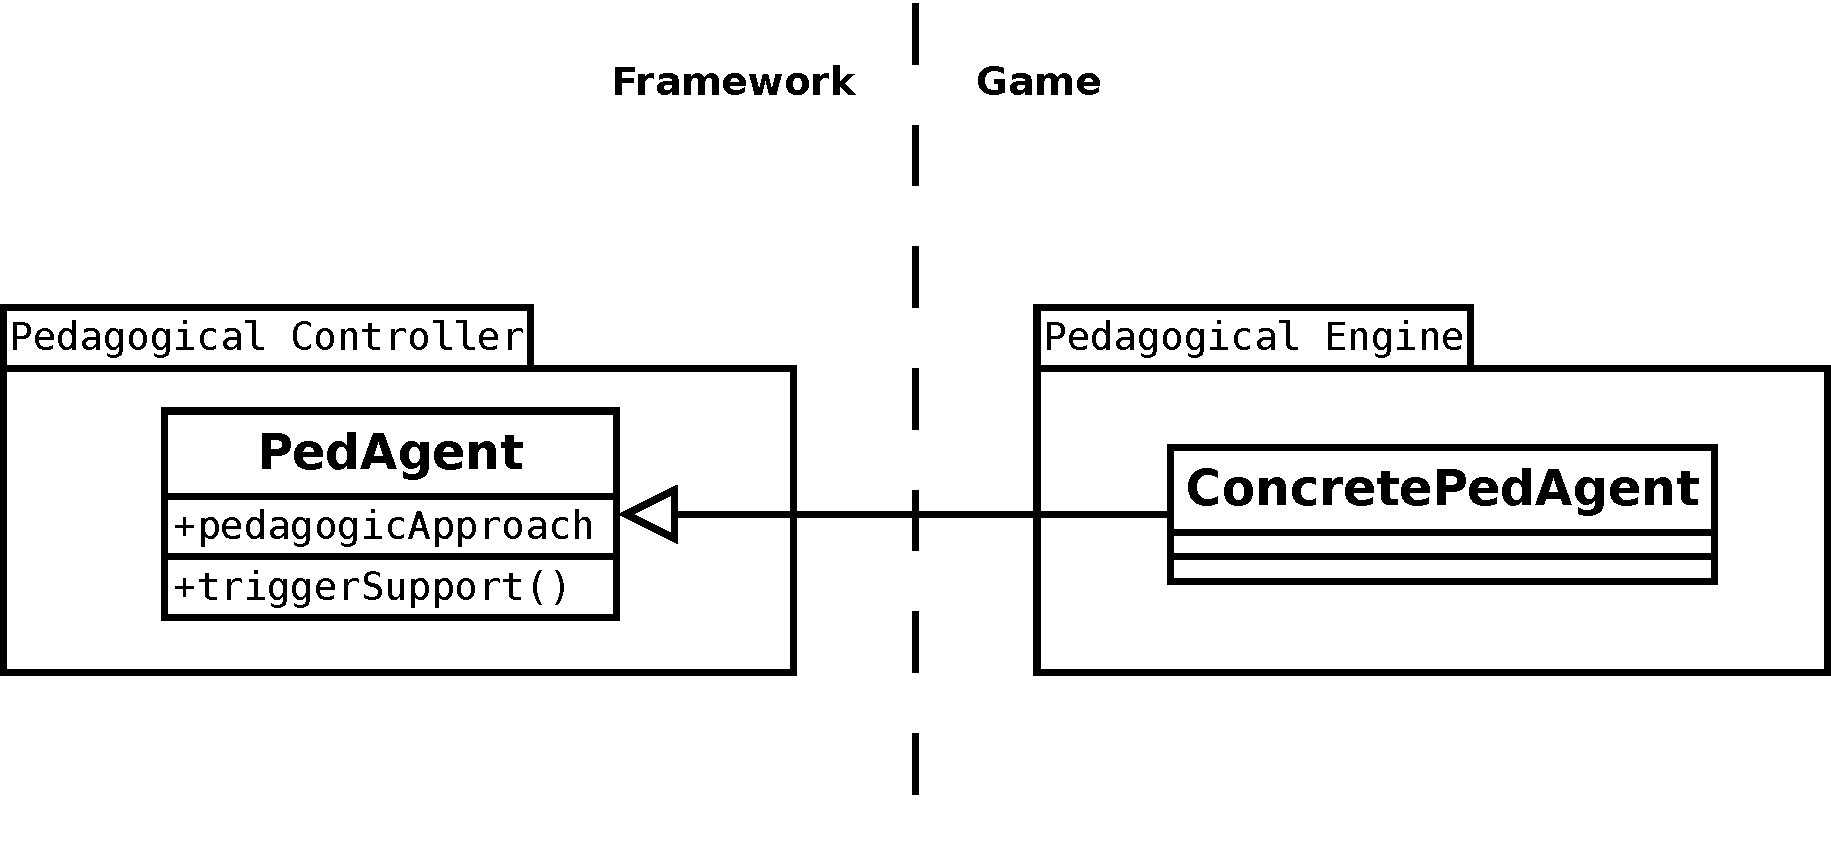
\includegraphics[width=0.8\textwidth]{diagrams/pedagent_concrete.pdf}
    \caption{The ConcretePedAgent implements the Abstract Class PedAgent (UML class diagram)}
\end{figure}
\end{frame}

\begin{frame}{Global Control Flow}
\begin{figure}
    \centering
    \includegraphics[width=\textwidth]{../latex/diagrams/global_control_flow_new.pdf}
    \caption{The Global Control Flow through the Subsystems (UML sequence diagram)}
\end{figure}
\end{frame}

\section{Outlook}

\subsection{Future Work}

\begin{frame}{Future Work}
\pause
\begin{itemize}
\item Define a language to describe interactions and patterns
\item Use AI / machine learning to learn interactions and patterns automatically
\item Research how children learn and how they behave during the process (needs interdisciplinary effort with pedagogues and psychologists)
\item Research and implement pedagogical agents
\item Evaluate
\end{itemize}
\end{frame}

\subsection{OLPC}

\begin{frame}{One Laptop Per Child}
\begin{itemize}
\item Non-profit organization
\item Kicked off at MIT Media Lab
\item Mission: ``bring education to the poorest children of the world''
\item Devices deployed until April 2009: 1.625 million
\item Perfect platform for ILF: open source, specialized software for children, high impact 
\end{itemize}
%\vspace{5mm}
\begin{figure}
    \centering
    
\includegraphics[width=0.4\textwidth]{images/OLPC_LOGO.png}
\end{figure}
\end{frame}

\begin{frame}{Contributors Program}
\begin{itemize}
\item Provide development devices (XO's) for contributors
\item Improve software - hardware usage
\item Inspire new projects
\end{itemize}
\pause
\begin{itemize}
\item Devices can be borrowed for a desired period of time
\item OLPC and developers should keep in touch -- support by a mentor
\item Publications, press reports, public relations, lending libraries
\end{itemize}
\pause
\begin{center}
{\color{blue} \footnotesize START A PROJECT THAT WILL CHANGE KIDS' LIVES WORLDWIDE!}
\end{center}
%\begin{block}{\tiny \centering START A PROJECT THAT WILL CHANGE KIDS' LIVES WORLDWIDE!}
\begin{figure}
    \centering
    
\includegraphics[width=0.3\textwidth]{images/Contributetree1.jpg}
\end{figure}
%\end{block}
\end{frame}

\section{Demo}

\subsection{Demo}
\begin{frame}
\huge
enjoy the demo...
\end{frame}

\subsection{Thanks}

\begin{frame}
\begin{center}
\huge
Thanks for the attention
\end{center}
\end{frame}

\appendix
\pagenumbering{Roman}

%%%%%%%%%%%%%%%%%%%%%%%%%%%%%%%%% Appendix %%%%%%%%%%%%%%%%%%%%%%%%%%%%%%%%%%%%%%%%%%

\section{Bibliography}
\begin{frame}[allowframebreaks]{Literature}
\tiny{\bibliography{../latex/bibtex/bachelor_thesis,../latex/bibtex/bachelor_thesis_2}}
\end{frame}

\section{Additional Material}
\begin{frame}{Use Case Overview}
\begin{figure}
    \centering
    \includegraphics[height=0.7\textheight]{../latex/diagrams/use_cases_overall.pdf}
    \caption{Overall use case diagram (UML use case diagram)}
\end{figure}
\end{frame}

\begin{frame}[allowframebreaks]{Object Design}
\begin{figure}
    \centering
    \includegraphics[height=0.5\textheight]{../latex/diagrams/InteractionPatterns.pdf}
    \caption{Matching Interactions to InteractionPatterns (UML class diagram)}
\end{figure}

\begin{figure}
    \centering
    \includegraphics[height=0.7\textheight]{../latex/diagrams/problemDetection.pdf}
    \caption{Problem Detection with Strategy Pattern (UML class diagram)}
\end{figure}
\end{frame}

\begin{frame}{Taxonomy}
\begin{figure}
    \centering
    \includegraphics[width=\textwidth]{../latex/diagrams/games_taxonomy.pdf}
    \caption[Taxonomy of Games (UML class diagram)]
    {Taxonomy of Games (UML class diagram)}
    \label{taxonomy_games}
\end{figure}
\end{frame}

\begin{frame}{Example}
\begin{block}{An example from a study in the US \cite{Bailey1982}:}
Setup: 4063 males, randomly selected from the US population\\
\vspace{5mm}
\pause
\begin{center}
\begin{tabular}{ r | c | c }
  Round & Probe size & Body dimension\\
  \hline
  0 & 4063 & initial probe \\
  1 & 1055 & standing height \\
  2 & 302 & chest circumference \\
  ... & ... & ... \\
  9 & 2 & arm length \\
 10 & 0 & -- \\
\end{tabular}
\end{center}
\end{block}
\end{frame}

\begin{frame}{Activity}
\begin{figure}
    \centering
    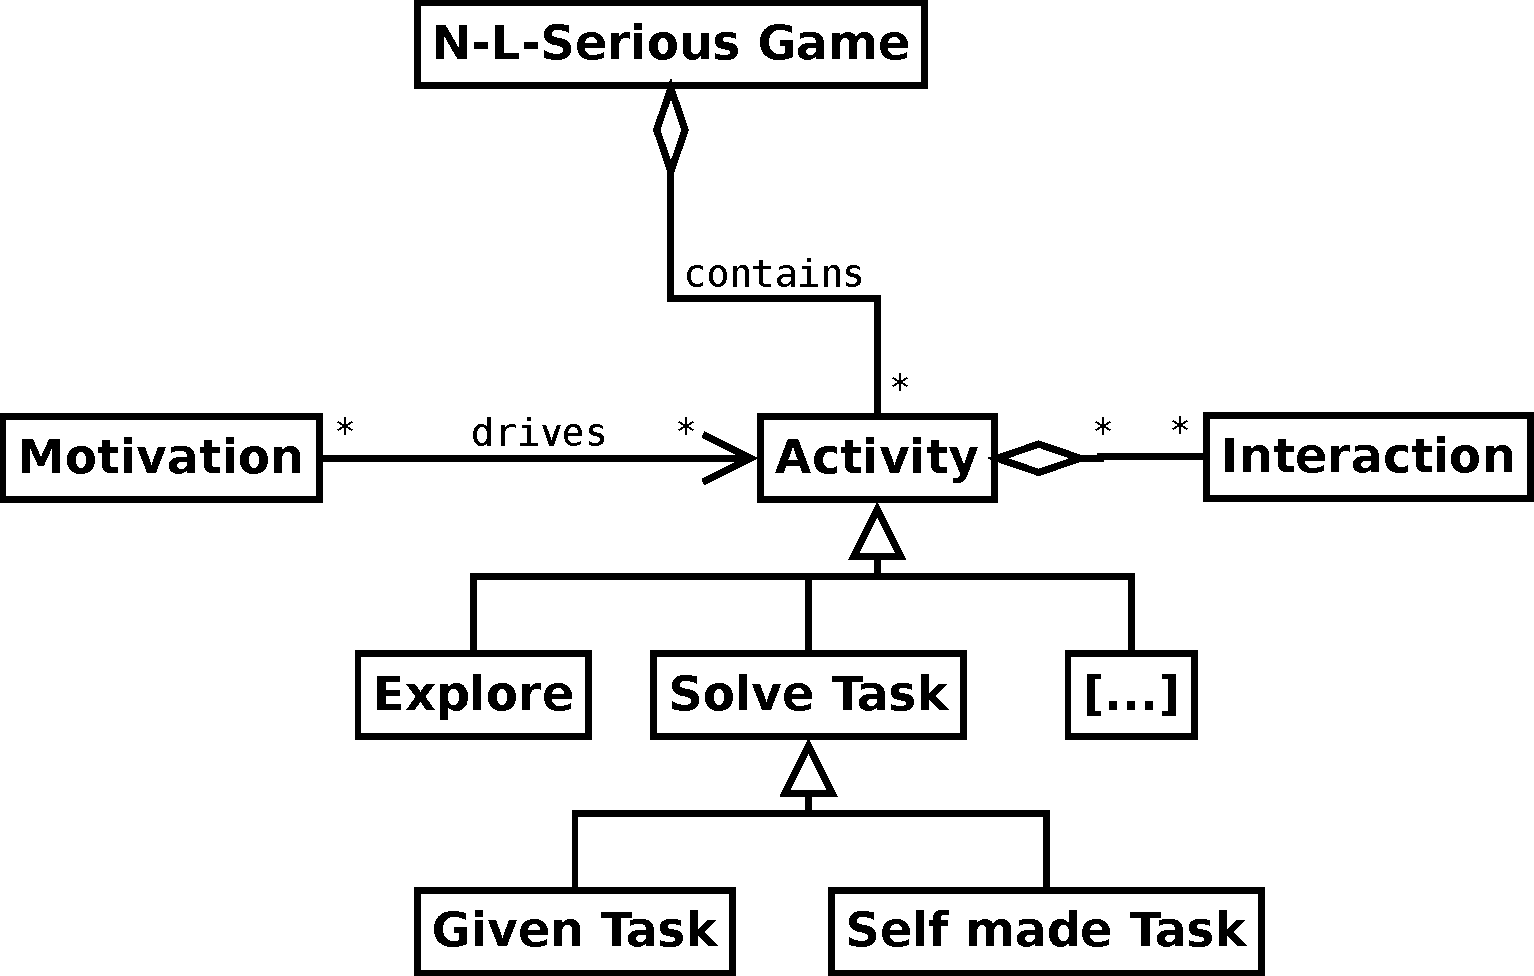
\includegraphics[height=0.6\textheight]{diagrams/activity_motivation.pdf}
    \caption{Different Activities in a Game (UML class diagram)}
\end{figure}
\end{frame}

\begin{frame}{Functional Requirements}
\begin{itemize}
\item Learner-Centric
\item Individual Support
\item Adaptive Learner Model
\item Task Independent Problem Detection
\end{itemize}
\end{frame}

\begin{frame}{Non Functional Requirements}
\begin{itemize}
\item Usability
\item Reliability
\item Performance
\item Supportability
\end{itemize}
\end{frame}

\end{document}
